\section{System Overview}
\label{sec:fdsp-tpcelec-overview}

%%%%%%%%%%%%%%%%%%%%%%%%%%%%%%%%%%%
\subsection{Introduction}
\label{sec:fdsp-tpcelec-overview-intro}

\todo{Mike M. will update section by November 23rd; currently using IDR text as placeholder}

DUNE single-phase time projection chamber TPC electronics hardware signal processing takes place inside the \lar, in boards that are directly mounted on the \dword{apa}; accordingly, the TPC readout electronics are referred to as the \dword{ce}.  The electronics are mounted inside the \lar to exploit the fact that charge carrier mobility in silicon is higher and that thermal fluctuations are lower at \lar temperature than at room temperature.  For \dword{cmos} (complementary metal-oxide-semiconductor) electronics, this results in substantially higher gain and lower noise at \lar temperature than at room temperature~\cite{larCMOS}.  Mounting the front-end electronics on the \dword{apa} frames also minimizes the input capacitance.  Furthermore, placing the digitizing and multiplexing (MUX) electronics inside the cryostat reduces the total number of penetrations into the cryostat and minimizes the number of cables coming out of the cryostat.  As the full TPC electronics chain for the \dword{spmod} includes many components on the warm side of the cryostat as well, the DUNE consortium designated to organize development of this system is called the DUNE \textit{Single-Phase TPC Electronics} consortium. It is sometimes referred to as the \dword{ce} consortium for short.
%\fixme{can we add (CE) here? Anne}

The overall noise requirement drives the choice of architecture of the TPC electronics. This requirement is difficult to establish precisely, but it is clear that the lower the electronic noise is, the greater the physics reach of the DUNE experiment will be.  An equivalent noise charge (\dword{enc}) of less than approximately 1000$e^-$ is required for satisfactory reconstruction of accelerator neutrino interactions, but a lower noise level will yield significantly better two-track separation and primary vertex resolution, and thus higher efficiency and/or lower background for identifying electron neutrino interactions.  Setting the noise level requirement for the DUNE \dword{spmod} more precisely is an ongoing effort.

The noise level enabled by having the front-end electronics in the cold (roughly half as much noise at \lar temperature than at room temperature) greatly extends the reach of the DUNE physics program.  Decreasing the noise level allows for smaller charge deposits to be measurable, which acts as a source of risk mitigation in the case that the desired drift field can not be reached or the electron lifetime in the detector is lower than desired (due to the electronegative impurities in the detector), and also increases the reach of low-energy physics measurements such as those associated with stellar core-collapse supernova burst neutrinos.  Finally, the low noise level allows the experiment to utilize low-energy $\mathrm{{}^{39}Ar}$ beta decays for the purpose of calibration in the DUNE \dword{spmod}.  The noise level requirement of \dword{enc}\,$<\num{1000}\,e^-$ will allow for the use of $\mathrm{{}^{39}Ar}$ beta decays in calibrations at the DUNE \dword{spmod}.

In order to retain maximum flexibility to optimize reconstruction algorithms after the DUNE data is collected, the \dword{spmod} electronics are designed to produce a digital record that is a representation of the waveform of the current produced by charge collection/induction on the anode wires.  Each anode wire signal is input to a charge sensitive amplifier, followed by a pulse shaping circuit and an \dword{adc}.  In order to minimize the number of cables and cryostat penetrations, the \dwords{adc} as well as the amplifier/shapers are located in the \lar, and digitized data from many wires are merged onto a much smaller set of high speed serial links.  %[Figure xx illustrates the front-end electronics architecture.  128-channel “Front-End Mother Boards” produce digitized waveforms and transmit those waveforms on four serial links through a \fdth in the top of the cryostat to “Warm Interface Boards” located in crates mounted directly on spool pieces on the outside of the cryostat. The Warm Interface Boards provide clean power and timing signals to the \dword{ce}.  All connections to the DAQ and slow control systems are made using optical fibers.] – might better cover later.

%INCLUDE AN OVERVIEW FIGURE HERE WITH THIS CAPTION:  ``Each Anode Plane Assembly (\dword{apa}) has 2560 instrumented wires.  These are read out by 20 Front-End MotherBoards (\dwords{femb}).  All cables between \dwords{femb} on a given \dword{apa} are routed through a single cryostat \fdth.  A printed circuit board connects those cables to the backplane of a Warm Electronics Interface Crate.  Warm Interface Boards mounted in this crate receive data from the \dwords{femb} and transmit it to the data acquisition system.''

%%%%%%%%%%%%%%%%%%%%%%%%%%%%%%%%%%%
\subsection{Design Considerations}
\label{sec:fdsp-tpcelec-overview-design}

\todo{Mike M. will update section by November 23rd; currently using IDR text as placeholder}

The \dword{ce} signal processing is implemented in application-specific integrated circuits (\dwords{asic})
using \dword{cmos} technology.  The \dword{ce} is continuously read out, resulting in a digitized \dword{adc}
sample from each \dword{apa} channel (wire) up to every \SI{500}{ns} (\SI{2}{MHz} sampling rate).

Each individual \dword{apa} has \num{2560} channels that are read out by \num{20} \dfirsts{femb}, with
each \dshort{femb} enabling digitized wire readout from \num{128} channels.  One cable bundle connects each \dshort{femb} to
the outside of the cryostat via a \dword{ce} signal cable flange located at the \dword{ce} \fdth at the
top of the cryostat, where a single flange services each \dword{apa}, as shown in Figure~\ref{fig:connections}.  Two \dword{ce} signal flanges are located on each \fdth, together accounting for all electronics channels associated with a pair of \dwords{apa} (upper and lower, vertically arranged).
Each cable bundle contains wires for low-voltage (\dword{lv}) power, high-speed data readout, and
clock or digital-control signal distribution.  Eight separate cables carry the TPC wire bias voltages
from the signal flange to the \dword{apa} wire bias boards, in addition to the bias voltages for the field
cage termination electrodes and for the electron diverters.  An additional flange on the top of each \fdth services the \dword{pds} cables associated with the \dword{apa} pair.

\begin{dunefigure}
[Connections between the signal flanges and \dword{apa}]
{fig:connections}
{Connections between the signal flanges and \dword{apa}. Only the upper \dword{apa} of the hanging \dword{apa} pair, described in Section~\ref{sec:fdsp-apa-frames}, and its connection paths are shown. The lower \dword{apa} shares the \dword{pd} flange with the upper \dword{apa} but has a separate TPC readout flange. A \textit{\dword{ce} module} consists of all \dword{ce} associated with \num{128} channels of digitized readout.}
%\hspace{1cm}
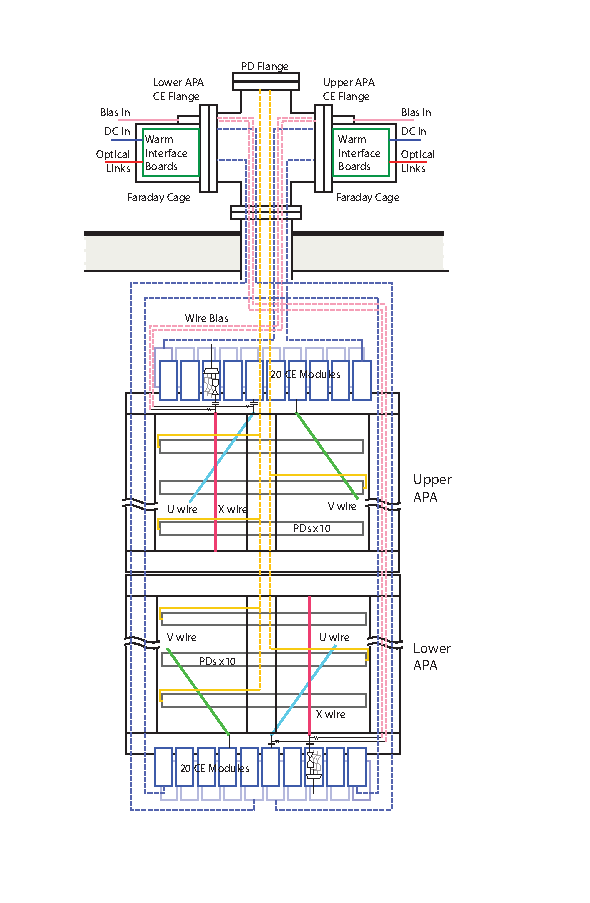
\includegraphics[width=0.9\textwidth]{sp-tpcelec-DUNE-FD-APA-readout-scheme-v1.pdf}
\end{dunefigure}

The components of the \dword{ce} system are the following:
\begin{itemize}
\item{\dwords{femb}, on which the \dwords{asic} are mounted, which are installed on the \dwords{apa};}
\item{cables for the data, clock and control signals, \dword{lv} power, and wire bias voltages between the \dword{apa} and the signal flanges (cold cables);}
\item{signal flanges with a \dword{ce} \fdth to pass the data, clock and control signals, \dword{lv} power, and \dword{apa} wire-bias voltages between the inside and outside of the cryostat, in addition to the corresponding cryostat penetrations and spool pieces;}
\item{%warm interface electronics crates (
\dwords{wiec} that are mounted on the signal flanges and contain
the %warm interface boards (
\dwords{wib} and %power and timing cards (
\dwords{ptc} for further processing
and distribution of the signals entering and exiting the cryostat;}
%\item{fiber cables for transmitting data and clock/control signals between the \dwords{wiec} and the
%data acquisition (DAQ) and slow control systems;}
\item{cables for \dword{lv} power and wire bias voltages between the signal flange and external power
supplies (warm cables); and}
\item{\dword{lv} power supplies for the \dword{ce} and bias-voltage power supplies for the \dwords{apa}.}
\end{itemize}

Table~\ref{tab:elecNums} lists the component type, the quantity required for each type  and the number of channels per component of each type.

\begin{dunetable}
[TPC electronics components and quantities for a single \dword{apa} of a %the DUNE \single 
\dword{spmod}.]
{llr}
{tab:elecNums}
{TPC electronics components and quantities for a single \dword{apa} of the DUNE \dword{spmod}.}
\textbf{Element} &\textbf{Quantity} & \textbf{Channels per element}\\ \toprowrule
Front-end mother board (\dword{femb}) & \num{20} per \dword{apa} & \num{128} \\ \colhline
FE \dword{asic} chip & \num{8} per \dword{femb} & \num{16} \\ \colhline
\dword{adc} \dword{asic} chip & \num{8} per \dword{femb} & \num{16} \\ \colhline
\dword{coldata} \dword{asic} chip & \num{2} per \dword{femb} & \num{64} \\ \colhline
Cold cable bundle & \num{1} per \dword{femb} & \num{128} \\ \colhline
Signal flange & \num{1} per \dword{apa} & \num{2560} \\ \colhline
\dword{ce} \fdth & \num{1} per \dword{apa} & \num{2560} \\ \colhline
Warm interface board (\dword{wib}) & \num{5} per \dword{apa} & \num{512} \\ \colhline
Warm interface electronics crate (\dword{wiec}) & \num{1} per \dword{apa} & \num{2560} \\ \colhline
Power and timing card (\dword{ptc}) & \num{1} per \dword{apa} & \num{2560} \\ \colhline
Power and timing backplane (PTB) & \num{1} per \dword{apa} & \num{2560} \\
%\dword{lv} power mainframe & ? & ? \\ \colhline
%\dword{lv} supply module & ? & ? \\ \colhline
%wire bias mini-crate & ? & ? \\ \colhline
%wire bias supply module & ? & ? \\
\end{dunetable}

The baseline design for the \dword{spmod} TPC electronics calls for three types of \dwords{asic} to be located inside of the \lar:
\begin{itemize}
\item{a \num{16}-channel \dword{fe} \dword{asic} for amplification and pulse shaping, referred to as \dword{larasic} in the following;}
\item{a \num{16}-channel \num{12}-bit \dword{adc} \dword{asic} operating at \SI{2}{MHz}; and}
\item{a \num{64}-channel control and communications \dword{asic}, referred to as \dword{coldata} in the following.}
\end{itemize}

The \dword{fe} \dword{asic} has been prototyped and is close to meeting requirements (discussed in Section~\ref{sec:fdsp-tpc-elec-ov-req}). Another prototype to address issues in the version deployed in \dword{pdsp} is expected in the spring of 2018. Key portions of the control and communications \dword{asic} (also referred to as the \dword{coldata} \dword{asic}) have been prototyped and meet requirements.  However, it has been determined that the BNL-designed P1-\dword{adc} \dword{asic} now being used in \dword{pdsp} does not meet requirements, and accordingly, its development has been terminated.  A new \dword{adc} \dword{asic} (referred to as the cold \dword{adc} \dword{asic}) is being developed by an LBNL-\fnal-BNL collaboration and first prototypes are expected by the end of summer 2018.  The first full prototype of the controls and communication \dword{asic} is also expected to be available for testing by the end of summer 2018. 

In order to maximize the probability of developing a complete design for cold TPC \dword{fe} electronics in a timely fashion, an alternative solution is also being investigated, a single \num{64}-channel \dword{asic} that will consolidate all three functions described above.  This design is being done at SLAC and first prototypes are expected in summer 2018.  An \dword{adc} solution in the form of a developmental \dword{adc} chip for an upgrade of the ATLAS detector provides an additional backup option; this option will be explored further if the performance of the other two \dword{adc} solutions being considered do not meet the requirements for DUNE.

While the higher charge carrier mobility at \lar temperature than at room temperature is central to the improved performance of \dword{ce}, it also leads to the \textit{hot carrier effect}.  In n-type MOS transistors, the carriers (electrons) can acquire enough kinetic energy to ionize silicon in the active channel.  This charge can become trapped and lead to effects (including threshold shifts) similar to those caused by radiation damage.  This effect can cause MOS circuits to age much more quickly at \lar temperature than at room temperature, reducing performance and potentially causing failure.  In order to mitigate this effect, the maximum \efield in transistor channels must be lower than the field that can be reliably used at room temperature.  
This is accomplished by using transistors that are fabricated with longer than typical length and operated at reduced bias voltage.  Any commercial circuits that are used in the \lar must be carefully tested to ensure that they will perform well for the expected \num{20}-year lifetime of DUNE.

A series of tests are planned to demonstrate that the \dword{ce} system design will meet DUNE requirements. These include two system tests: one using the \dword{pdsp} \textit{cold box} at CERN, and one using a new small \lartpc at \fnal. The latter will also accommodate one half-length DUNE \dword{pd}, and will provide a low-noise environment that will allow one to make detailed comparisons of the performance of the new \dwords{asic}. It will also enable the study of interactions between the TPC readout and other systems, including the \dword{pd} readout and the \dword{hv} distribution. These test facilities are discussed in more detail in Section~\ref{sec:fdsp-tpc-elec-qa-facilities}. Plans are also being made for a second period of data taking for the \dword{pdsp} detector, with final \dwords{apa} including the final \dwords{asic} and \dwords{femb} replacing the current prototypes. This second run of \dword{pdsp} is planned for 2021-2022.

%%%%%%%%%%%%%%%%%%%%%%%%%%%%%%%%%%%
\subsection{Scope and Requirements}
\label{sec:fdsp-tpcelec-overview-scope}

\todo{Mike M. will update section by November 23rd; currently using IDR text as placeholder}

In addition to the noise requirement (less than \num{1000}\,$e^{-}$), several additional requirements determine most of the other important TPC electronics specifications.  These are:

\begin{itemize}
\item{The \dword{fe} peaking time must  %should 
be  in the range \numrange{1}{3}\,\si{\micro\second}.  This requirement is derived primarily from the time required for drifting charges to travel from one plane of anode wires to the next.}
\item{The \dword{fe} must %should 
 have an adjustable baseline.  This requirement reflects the fact that the signal from induction wires is bipolar while the signal from the collection wires is mostly unipolar.}
\item{The \dword{adc} sampling frequency must %should 
be \SI{2}{MHz}.  This value is chosen to match a \dword{fe} shaping time of \SI{1}{\micro\second} (approximate Nyquist condition) while minimizing the data rate.}
\item{The system must 
have a linear response up to an impulse input of at least \num{500000}\,$e^{-}$.  This roughly corresponds to the charge collected on a single wire from one stopping proton and two more highly ionizing protons, all assumed to have trajectories at \num{45}\,$^{\circ}$ with respect to the beam axis.  This number was chosen so that saturation will occur in less than \SI{5}{\%} of beam related events.  Studies are ongoing (including an evaluation of \lariat~\cite{Cavanna:2014iqa} data and simulation studies) to better understand this requirement.}
\item{The dynamic range of the system must be at least \num{3000}:\num{1}. This number is given by the ratio between the maximum signal for no saturation and 50\% of the lowest possible noise level.  It implies a \num{12}-bit \dword{adc}.}
\item{The \dword{adc} must not contribute significantly to overall \dword{fe} noise. This requirement is dependent on the gain of the \dword{fe}, but for each gain setting translates into requirements on \dword{adc} parameters including non-linearity and noise.}
\item{The power dissipated by the electronics located in the \lar must 
be less than \SI{50}{mW/channel}.  Lower power dissipation is desirable because the mass of the power cables scales with the power.  Studies are ongoing to understand if the amount of power dissipated by the electronics should be minimized further due to potential complications from argon boiling; in principle this should not be a problem because the \dword{ce} boxes housing the \dwords{femb} are designed to channel bubbles to the \dword{apa} frames.}
\end{itemize}

Finally, all electronics located in the \lar must 
be highly reliable because it will not be possible to access the \dword{ce} for repair once the cryostat is filled with \lar. Studies are ongoing to quantify the impact of failures in the TPC and electronics, including single wire failures, and failures of groups of \num{16}, \num{64}, or \num{128} channels.

%%%%%%%%%%%%%%%%%%%%%%%%%%%%%%%%%%%
\subsection{ProtoDUNE-SP Results}
\label{sec:fdsp-tpcelec-overview-pdune}

The Single Phase ProtoDUNE-SP detector, described in Section~\ref{protodune-overview}, is a 700~ton fiducial volume LArTPC with 15,360 sense wires which are read out by a cold electronics (CE) system described in Section~\ref{sec:fdsp-tpcelec-qa-facilities-pdune}. It was deployed in a beam line of the CERN Neutrino Platform in 2018 and continued to take cosmic event data into 2019. The goal for the ProtoDUNE-SP TPC readout was to validate the concept and design of the integrated APA+CE readout and measure the performance of the CE system with components as close as possible to the final DUNE TPC readout.

Each of the six ProtoDUNE-SP APA+CE readout unit consists of 2,560 sense wires, of which 960 are 6.0~meter long collection wires and 1,600 are 7.4~meter long induction wires. Each one was tested in a full scale ``Cold Box'' in cold gaseous Nitrogen (GN2) with a complete CE readout system identical to the one on the detector prior to installation in the cryostat. Figure~\ref{fig:apa2-cycle} shows the Equivalent Noise Charge (ENC), which is the charge in electrons that would have to arrive at the sense wires to generate a signal with the RMS measured by the Front-End electronics, as a function of cold cycle time. At a stable temperature of 160 Kelvin the ENC for all 3 wire planes is below 500~e$^-$.

\begin{dunefigure}
[\dword{pdsp} APA2 noise levels measured in GN2 at CERN Cold Box]
{fig:apa2-cycle}
{Left Y-axis: ENC (in electrons) for U, V and X (red, blue and green curves) sense wire planes as a function of time (hours) for the APA2 cold cycle in GN2 in the CERN Cold Box; right Y-axis: temperature (orange curve) measured at the level of the Front-End electronics.}
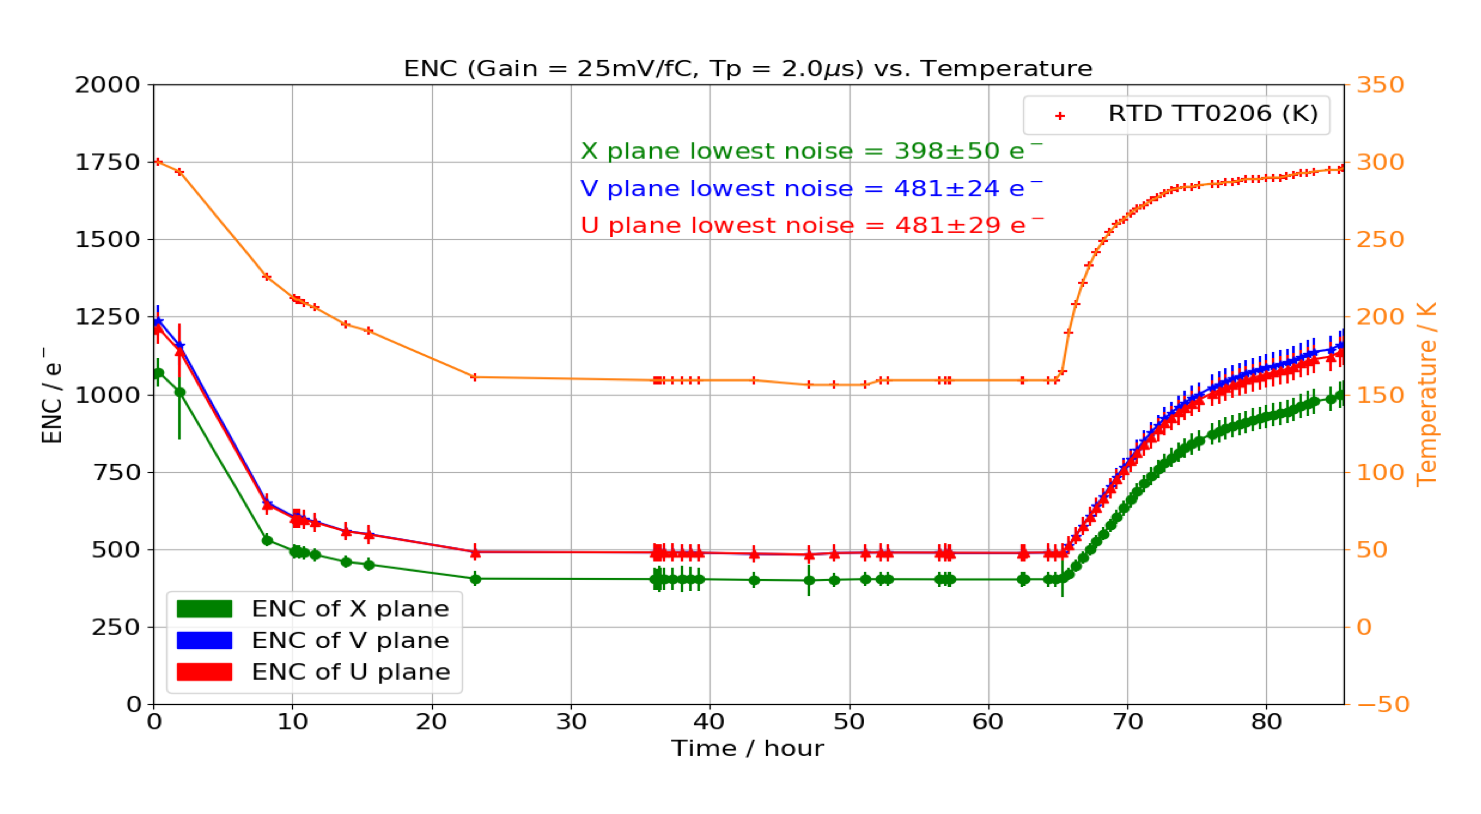
\includegraphics[width=1.0\linewidth]{sp-tpcelec-apa2.png}
\end{dunefigure}

After the cryostat was filled with LAr and the drift and wire bias HV were set to nominal (defined in Section~\ref{protodune-overview}), 99.7\% of the TPC readout channels were alive. The following channels were expected to be unresponsive to charge deposited on the wires:
\begin{itemize}
\item 4 electronics channels, suggesting a dead channel in the electronics, all on collection wires on three different APAs;
\item $\sim$35 channels were measured with ENC consistent with no capacitive load on the Front-End (FE) electronics, suggesting an open connection somewhere in front of the CE system, scattered randomly throughout the detector and on all wire planes.
\end{itemize}
With the detector in nominal operating conditions, the ENC was found to be $\sim$550~e$^-$ on the collection wires and $\sim$750~e$^-$ averaged over all operational channels. Figure~\ref{fig:apa3-noise} shows the ENC in electrons for all channels of one of the APA+CE readout units. The collection channels with ENC$>$1500~e$^-$ are caused by an artifact in the generation of cold ADC ASIC used in ProtoDUNE-SP. The channels in all three planes with ENC$<$300~e$^-$ have an open connection somewhere in front of the CE system.

\begin{dunefigure}
[TPC noise levels measured at \dword{pdsp} after \lar fill]
{fig:apa3-noise}
{ENC (in electrons) for all U, V and X (red, blue and green curves) sense wire planes for one ProtoDUNE APA with the detector in nominal operating conditions.}
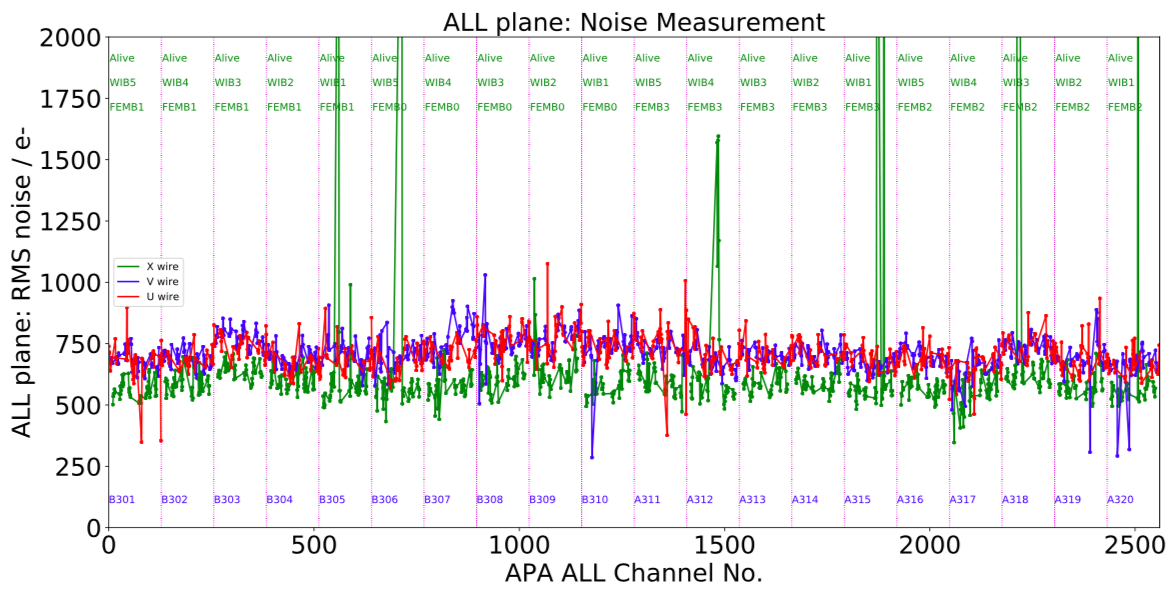
\includegraphics[width=1.0\linewidth]{sp-tpcelec-apa3-enc.png}
\end{dunefigure}

The overall performance of the CE system in ProtoDUNE-SP satisfies the DUNE single phase Far Detector CE system requirements listed in Section~\ref{sec:fdsp-tpcelec-overview-scope}. The overall system architecture, described in Section~\ref{sec:fdsp-tpcelec-overview-design}, will remain the same for the DUNE Cold Electronics. However, several improvements and updates to the CE system design motivated by the results from the testing and commissioning of, and the data-taking with, the ProtoDUNE-SP electronics will be discussed in this chapter.
